\documentclass{beamer}
\usetheme{metropolis}
\usepackage{graphicx}
\usepackage{subfig}
\usepackage{tcolorbox}
\title{Calculus-Based Physics-2: Electricity and Magnetism (PHYS180-02): Unit 2}
\author{Jordan Hanson}
\institute{Whittier College Department of Physics and Astronomy}

\begin{document}
\maketitle

\section{Unit 1 Review}

\begin{frame}{Unit 1 Summary}
\textbf{Reading: Chapters 5-6}
\begin{enumerate}
\item Charge, Conductors and Insulators
\item Coulomb's Law and Electric Fields
\item E-fields of Charge Distributions
\item Gauss's Law
\end{enumerate}
\end{frame}

\section{Unit 1 Review Problems}

\begin{frame}{Unit 3 Review Problems}
Suppose a charge $q$ is located at the origin.  Use Gauss' law to find the electric field.  What is the electric field?
\begin{itemize}
\item A: $\vec{E} = \frac{kq}{r}\hat{r}$
\item B: $\vec{E} = \frac{kq}{r^2}\hat{r}$
\item C: $\vec{E} = \frac{kq}{r^3}\hat{r}$
\item D: $\vec{E} = \frac{kq^2}{r^2}\hat{r}$
\end{itemize}
\end{frame}

\begin{frame}{Unit 3 Review Problems}
Suppose a line of charge runs up the z-axis.  The charge per unit length is $\lambda$.  Use Gauss' law to find the electric field.  What is the electric field at a point $P = (x,0,0)$?
\begin{itemize}
\item A: $\vec{E} = \frac{2k\lambda}{r^2} \hat{x}$
\item B: $\vec{E} = \frac{2k\lambda^2}{r^2} \hat{x}$
\item C: $\vec{E} = \frac{2k\lambda}{r} \hat{x}$
\item D: $\vec{E} = 0$
\end{itemize}
\end{frame}

\section{Summary}

\begin{frame}{Unit 4 Summary}
\textbf{Reading: Chapters 7-8}
\begin{enumerate}
\item Voltage
\begin{enumerate}
\item Review of work and energy
\item Review of conservative forces
\end{enumerate}
\item Capacitance
\end{enumerate}
\end{frame}

\section{Voltage}

\begin{frame}{Voltage}
\alert{Voltage} is analogous to potential energy in electrostatics.  The negative derivative of potential energy U is the force F:
\begin{equation}
F = -\frac{dU}{dx}
\end{equation}
For example, if the force is $F = -mg$, and the potential energy is $U = mgy$, then 
\begin{equation}
\frac{dU}{dy} = -mg
\end{equation}
\end{frame}

\begin{frame}{Voltage}
\alert{Voltage} is analogous to potential energy in electrostatics.  The derivative of voltage V is the field E:
\begin{equation}
E = -\frac{dV}{dx}
\end{equation}
For example, if the field is $E = \sigma/\epsilon_0$, and the potential energy is $V = \sigma/\epsilon_0 x + C$, then 
\begin{equation}
\frac{dV}{dx} = \sigma/\epsilon_0
\end{equation}
\end{frame}

\begin{frame}{Voltage}
\alert{Voltage} is analogous to potential energy in electrostatics. \\ \vspace{1cm}
Potential energy is just an energy.  A \textit{potential} in mechanics is the potential energy per unit mass.  \textit{Voltage}, or \textit{electrostatic potential} is \textbf{\alert{potential energy per unit charge.}} \\ \vspace{0.5cm}
The Volt (V) is the unit of voltage, and it has units of 1 V = 1 J/C.
\end{frame}

\begin{frame}{Voltage}
\textbf{Group board exercise}: Show that the units of electric field (normally Newtons per Coulomb) are also Volts per meter.
\end{frame}

\begin{frame}{Voltage}
\small
If the potential energy is a function of displacement, $U = U(\vec{x})$, it may be called a potential energy \textit{surface}.
\begin{figure}
\centering
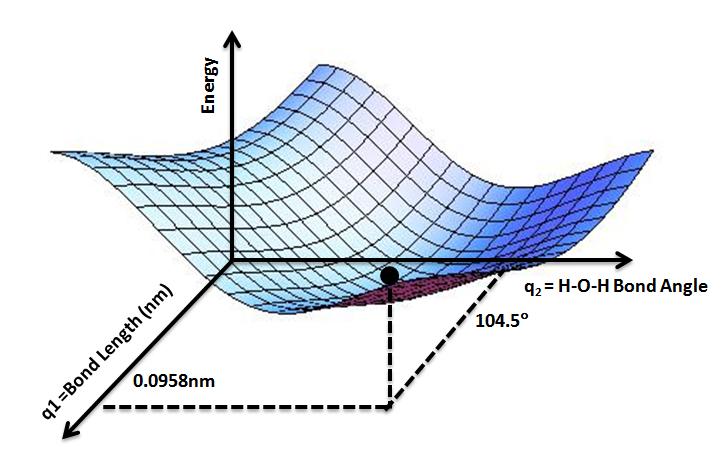
\includegraphics[width=0.5\textwidth]{figures/potential.png}
\caption{\label{fig:potential} An example of a potential energy surface.}
\end{figure}
\end{frame}

\begin{frame}{Voltage}
\small
Considering \textit{Newton's Second Law}, however, if $F = m a$ then $m a = -\frac{\Delta U}{\Delta x}$, and
\begin{equation}
a = -\frac{1}{m}\frac{\Delta U}{\Delta x} \label{eq:field}
\end{equation}
\begin{figure}
\centering
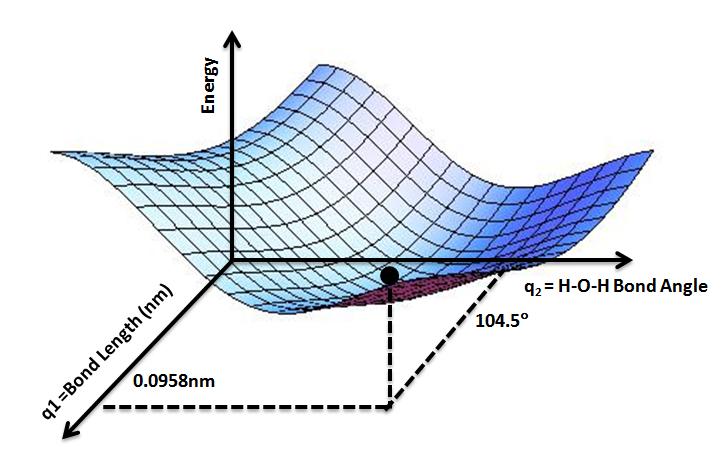
\includegraphics[width=0.4\textwidth]{figures/potential.png}
\caption{\label{fig:potential2} If we divide by the mass we have acceleration.}
\end{figure}
The derivative, or \textit{gradient}, of $a$ in Eq. \ref{eq:field} is analogous to the electric field.  But the electric field is a \textit{vector field}...
\end{frame}

\begin{frame}{Voltage}
The gradient is like a derivative, but gives you the proper direction wherever you are.
\begin{equation}
\boxed{
-\vec{\nabla} V = \vec{E} = -\frac{\partial V}{\partial x}\hat{i}-\frac{\partial V}{\partial y}\hat{j}-\frac{\partial V}{\partial z}\hat{k}}
\end{equation}
\end{frame}

\begin{frame}{Unit 3 Review Problems}
Suppose the voltage due to some charge distribution is $V(x,y,z) = ax+b$.  What is the field?
\begin{itemize}
\item A: $\vec{E} = a\hat{j}$
\item B: $\vec{E} = a\hat{k}$
\item C: $\vec{E} = b\hat{i}$
\item D: $\vec{E} = -a\hat{i}$
\end{itemize}
\end{frame}

\begin{frame}{Unit 3 Review Problems}
Suppose the voltage due to some charge distribution is $V(x,y,z) = ax+by$.  What is the field?
\begin{itemize}
\item A: $\vec{E} = -a\hat{j}-b\hat{j}$
\item B: $\vec{E} = a\hat{k}+b\hat{k}$
\item C: $\vec{E} = -b\hat{i}-a\hat{j}$
\item D: $\vec{E} = -a\hat{i}-b\hat{j}$
\end{itemize}
\end{frame}

\begin{frame}{Voltage}
Suppose a charge distribution is made of two infinite plates of charge with charge per unit area $\pm\sigma$.  We know that the field is $\sigma/\epsilon_0 \hat{k}$ between them.  \textbf{Group board exercise}: Draw the charge distribution, define a coordinate system, and write the function for the voltage.
\end{frame}

\begin{frame}{Voltage}
\textbf{Voltage} is like a potential energy surface $\rightarrow$ \textit{potential energy per unit charge.} \\ \vspace{0.5cm}
\url{https://phet.colorado.edu/en/simulation/charges-and-fields} \\
\alert{Using the PhET simulation about charges and fields}:
\begin{enumerate}
\item Explore the voltage associated with fields generated by charges using the voltage button.
\item Add a single point charge, and use the ruler and voltmeter (potentiometer) to measure voltage versus distance, and plot it.
\item What function describes the relationship between voltage and distance?
\end{enumerate}
\end{frame}

\begin{frame}{Voltage}
\url{https://phet.colorado.edu/en/simulation/charges-and-fields} \\
\alert{Using the PhET simulation about charges and fields}:
\begin{enumerate}
\item Note that the units of $\epsilon_0$ are N m$^2$ C$^{-2}$, and the value is $8.854\times 10^{-12}$
\item We know from prior equations that the units of voltage are J C$^{-1}$
\item Using your measurements, show that the voltage due to a point charge is
\begin{equation}
\boxed{
V = \pm \frac{1}{4\pi \epsilon_0} \frac{q}{r}}
\end{equation}
(Where the sign depends on the charge, just like E-fields)
\end{enumerate}
\end{frame}

\begin{frame}{Voltage}
Voltage due to a point charge:
\begin{equation}
\boxed{
V = \pm \frac{1}{4\pi \epsilon_0} \frac{q}{r}} \label{eq:volt2}
\end{equation}
\end{frame}

\begin{frame}{Voltage}
Voltage is an example of a \textbf{scalar field}, whereas the electric field is an example of a \textbf{vector field.}  Create two lines of charge, one positive and one negative in the PHeT simulator, and pretend they represent planes of charge coming out of the screen.  The field should constant and uniform like
\begin{equation}
\vec{E} = \frac{\sigma}{\epsilon_0} \hat{k}
\end{equation}
\begin{enumerate}
\item Plot the voltage versus distance between the plates.
\item Calculate the slope in V/m, and the y-intercept in V.
\item Does the electric field depend on the y-intercept?  Does the charge distribution?
\end{enumerate}
\end{frame}

\begin{frame}{Voltage}
\begin{figure}
\centering
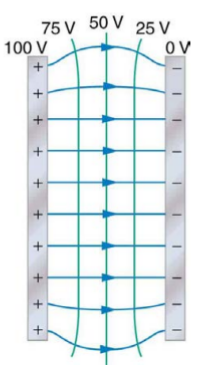
\includegraphics[width=0.25\textwidth]{figures/plates.png}
\caption{\label{fig:plates} Parallel plates of charge, electric field, and potential.  Notice the linear decrease in voltage.}
\end{figure}
\textbf{How we define the y-intercept in voltage is analogous to the zero-point freedom of potential energy.}
\end{frame}

\begin{frame}{Voltage}
\textit{Two parallel plates, opposite charge}:
\begin{equation}
V = -\frac{\sigma}{\epsilon_0}z + C
\end{equation}
With the boundary condition that $V = V_0$ when $z = 0$, we have
\begin{equation}
V(z) - V_0 = -\frac{\sigma}{\epsilon_0}z
\end{equation}
Let $\Delta V(z) = V(z) - V_0$, and $\Delta z = z$:
\begin{equation}
-\frac{\Delta V}{\Delta z} = \frac{\sigma}{\epsilon_0} =  E
\end{equation}
\end{frame}

\begin{frame}{Voltage}
\textbf{Continuing with PHeT:} Make a ring of charge that has a radius of 100 cm, with the center at the origin.
\begin{enumerate}
\item Show that the voltage field is radially symmetric.
\begin{itemize}
\item Place \textit{equipotential lines} around the charge distribution and see that they are circular.
\end{itemize}
\item Show that at distances much larger than the radius, the voltage field looks like that of a point charge.
\begin{itemize}
\item Record the voltage versus distance from the origin.
\item Plot the data.
\item Compare to the plot corresponding to a point charge.
\end{itemize}
\end{enumerate} 
\end{frame}

\section{Units of Energy}

\begin{frame}{Units of Energy}
The electron-volt: eV.  This is the energy gained by an electron accelerated through a voltage of 1 V.
\begin{itemize}
\item How many Joules per electron volt?
\item What is the mass of a proton in eV? (E = mc$^2$, where $c$ is the speed of light.)
\end{itemize}
\end{frame}

\begin{frame}{Units of Energy}
A proton is released into a 40 kV electric potential.  What is the final kinetic energy of the proton?
\begin{itemize}
\item A: -20 kV
\item B: 40 kV
\item C: -40 keV
\item D: 40 keV
\end{itemize}
\end{frame}

\begin{frame}{Units of Energy}
An alpha particle is a helium nucleus with a charge of $+2 q_e$.  Suppose an alpha particle is accelerated and has a final energy of 2 MeV.  How many volts were required to accelerated it?
\begin{itemize}
\item A: 4 MV
\item B: 3 MV
\item C: 2 MV
\item D: 1 MV
\end{itemize}
\end{frame}

\begin{frame}{Units of Energy}
\begin{figure}
\centering
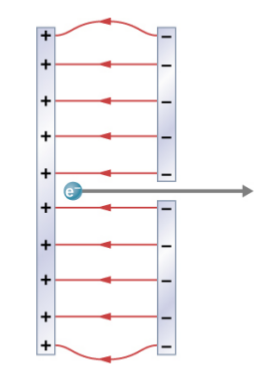
\includegraphics[width=0.3\textwidth]{figures/accel_plates.png}
\caption{\label{fig:accel_plate} An electron accelerated by a parallel plate capacitor.}
\end{figure}
\end{frame}

\begin{frame}{Units of Energy}
An electron has a charge $-q_e$.  Suppose an electron is accelerated through a voltage of 1 V toward another electron at a fixed position.  How close does the moving electron get to the stationary one?
\begin{itemize}
\item A: about 0.1 nm
\item B: about 1 nm
\item C: about 10 nm
\item D: about 100 nm
\end{itemize}
\end{frame}

\begin{frame}{Units of Energy}
A bare helium nucleus has two positive charges and a mass of $6.64 \times 10^{-27}$ kg.  What is the kinetic energy at 2 percent of the speed of light?  The speed of light is $c = 3.0 \times 10^{8}$ m/s.
\begin{itemize}
\item A: $1.2 \times 10^{-10}$ J
\item B: $1.2 \times 10^{-11}$ J
\item C: $1.2 \times 10^{-12}$ J
\item D: $1.2 \times 10^{-13}$ J
\end{itemize}
\end{frame}

\begin{frame}{Units of Energy}
What is the previous energy in eV?
\begin{itemize}
\item A: 0.75 MeV
\item B: 0.75 keV
\item C: 0.75 GeV
\item D: 0.75 eV
\end{itemize}
\end{frame}

\begin{frame}{Units of Energy}
Remember that this is an alpha particle (helium nucleus) with a +2 charge.  How many volts are required to give it an energy of 0.75 MeV?
\begin{itemize}
\item A: 0.375 MV
\item B: 0.75 MV
\item C: 1.5 MV
\item D: 0.375 V
\end{itemize}
\end{frame}

\section{Capacitance}

\begin{frame}{Capacitance}
\textbf{Capacitance} is the ability of an object to store charge.  Let the voltage difference across an object be $V$, storing $-Q$ on one side and $+Q$ on another.  The \textit{capacitance} $C$ is given by
\begin{equation}
Q = C V
\end{equation}
Let the object be two parallel plates, and the charges be $\pm Q$.
\end{frame}

\begin{frame}{Capacitance}
\begin{figure}
\centering
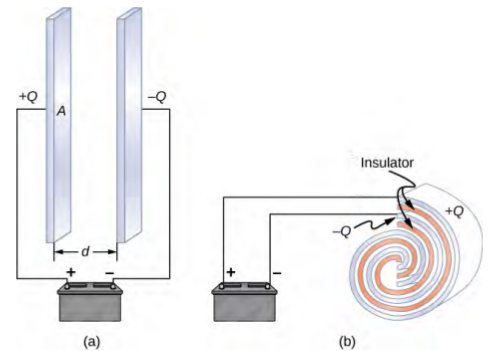
\includegraphics[width=0.8\textwidth]{figures/cap.png}
\caption{\label{fig:cap} General scheme of a capacitor.}
\end{figure}
\end{frame}

\begin{frame}{Capacitance}
The electric field and voltage between two charged plates separated by a distance $d$ is $V = Ed$.  The field is $E = \sigma/\epsilon_0$, and $Q = \sigma/A$, where $A$ is the plate area and $\sigma$ is the surface charged density.  Note that
\begin{align}
C = Q/V &= (Q)/(E d) \\
= (Q \epsilon_0)/(\sigma d) &= (Q A \epsilon_0)/(Q d) \\
= \frac{A \epsilon_0}{d} &
\end{align}
So the capacitance depends on the permittivity of free space, the area, and the distance.  In other words, just the geometry of the system.  The units of capcitance are \textbf{\alert{Farads}} (F).  This is a large unit.  Typical capacitors have nF or pF.
\end{frame}

\begin{frame}{Capacitance}
\textbf{Group board exercise}: The permittivity of free space is $8.85 \times 10^{-12}$ N$^{-1}$ C$^2$ m$^{-2}$.  A capacitor has an area of 1 mm$^2$, and $d = 0.001$ mm.  What is the capacitance? \\ 
\textbf{Group board exercise}: The permittivity of free space is $8.85 \times 10^{-12}$ N$^{-1}$ C$^2$ m$^{-2}$.  A capacitor has an area of 10 mm$^2$, and $d = 0.001$ mm.  What is the capacitance? \\
\textbf{Group board exercise}: The permittivity of free space is $8.85 \times 10^{-12}$ N$^{-1}$ C$^2$ m$^{-2}$.  A capacitor has an area of 1 mm$^2$, and $d = 0.01$ mm.  What is the capacitance?
\end{frame}

\section{Capacitors in series and in parallel}

\begin{frame}{Capacitors in series and in parallel}
\textbf{Observe on board.}
\begin{enumerate}
\item Consider two capacitors \textit{in series,} with capacitance $C_1$ and $C_2$.  What is the total capacitance?
\item Consider two capacitors \textit{in parallel,} with capacitance $C_1$ and $C_2$.  What is the total capacitance?
\end{enumerate}
\textbf{Create a simple circuit with capacitors}, and a battery to charge them.  How much total charge is stored?  Exchange your design with another group, and solve each others' problem.
\end{frame}

\section{Ohm's Law, Kirchhoff's Rules and Simple Circuits}

\begin{frame}{Ohm's Law, Kirchhoff's Rules and Simple Circuits}
\textbf{Read chapters 9 and 10 for Monday.}
Voltage and capacitance can be combined with another concept, \alert{resistance}, to build an understanding of \alert{circuits}.  Ohm's law is the relationship between \textit{current} and \textit{voltage}:
\begin{equation}
V = I R = \frac{dQ}{dt}R
\end{equation}
Current is the \textit{flow of charge.}  The unit of resistance is called the Ohm, and the unit of current is called the amp, for Amp\`{e}re.
\end{frame}

\begin{frame}{Ohm's Law, Kirchhoff's Rules and Simple Circuits}
A 9 V battery powers a smoke detector, and the current is 0.009 amps.  What is the resistance of the circuit powering the smoke detector?
\begin{itemize}
\item A: 1000 Ohms
\item B: 100 Ohms
\item C: 10 Ohms
\item D: 1 Ohm
\end{itemize}
\end{frame}

\begin{frame}{Ohm's Law, Kirchhoff's Rules and Simple Circuits}
A 3.3 V battery powers a christmas light, and the current is 0.33 amps.  What is the resistance of the circuit powering the smoke detector?
\begin{itemize}
\item A: 1000 Ohms
\item B: 100 Ohms
\item C: 10 Ohms
\item D: 1 Ohm
\end{itemize}
\end{frame}

\begin{frame}{Ohm's Law, Kirchhoff's Rules and Simple Circuits}
Resistors, capacitors, voltages, and current can be combined conceptually to form \alert{\textbf{DC Circuits}} (direct-current).  The following rules govern the interaction of resistors with each other, and capacitors with each other:
\begin{itemize}
\item For resistors \textit{in series}: $R = R_1 + R_2 + R_3 + ...$
\item For resistors \textit{in parallel}: $R^{-1} = R_1^{-1} + R_2^{-1} + R_3^{-1} + ...$
\item For capacitors \textit{in parallel}: $C = C_1 + C_2 + C_3 + ...$
\item For capacitors \textit{in series}: $C^{-1} = C_1^{-1} + C_2^{-1} + C_3^{-1} + ...$
\end{itemize}
\textbf{Observe on board:} difference between in series, and in parallel? (Hint, different voltage for in series, same voltage for in parallel).
\end{frame}

\begin{frame}{Ohm's Law, Kirchhoff's Rules and Simple Circuits}
Kirchhoff's rules:
\begin{enumerate}
\item Summing the voltage in a loop must equal zero ($\vec{E}$-fields are conservative).
\item Current entering an leaving a node is conserved.
\end{enumerate}
\textbf{Observe on board.}
\end{frame}

\begin{frame}{Ohm's Law, Kirchhoff's Rules and Simple Circuits}
Two resistors have 1 k$\Omega$ each (1000 Ohms).  What is the effective resistance if they are added \textit{in parallel}?
\begin{itemize}
\item A: 1000 Ohms
\item B: 500 Ohms
\item C: 2000 Ohms
\item D: 200 Ohms
\end{itemize}
\end{frame}

\begin{frame}{Ohm's Law, Kirchhoff's Rules and Simple Circuits}
Two capacitors have 1 nF each.  What is the effective capacitance if they are added \textit{in series}?
\begin{itemize}
\item A: 0.5 nF
\item B: 5 nF
\item C: 1 nF
\item D: 2 nF
\end{itemize}
\end{frame}

\begin{frame}{Ohm's Law, Kirchhoff's Rules and Simple Circuits}
Two capacitors have 1 nF each.  What is the effective capacitance if they are added \textit{in parallel}?
\begin{itemize}
\item A: 0.5 nF
\item B: 5 nF
\item C: 1 nF
\item D: 2 nF
\end{itemize}
\end{frame}

\section{Graphical Analysis of Simple Circuits}

\begin{frame}{Graphical Analysis}
\begin{columns}[T]
\begin{column}{0.5\textwidth}
\begin{figure}
\centering
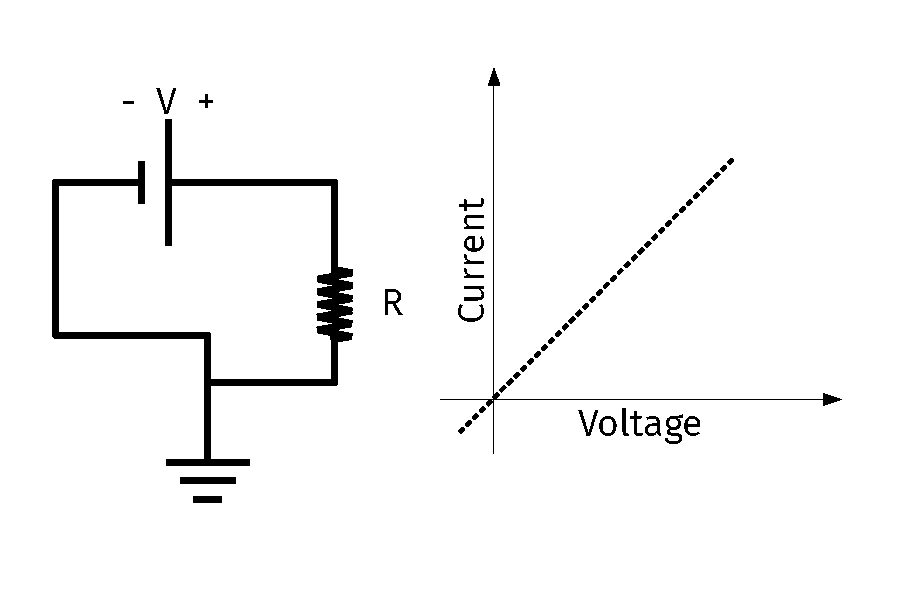
\includegraphics[width=\textwidth,trim=0.5cm 0cm 1cm 0cm,clip=true]{figures/iVCurve.pdf}
\caption{\label{fig:iVCurve1} Circuits components are represented graphically by iV curves.}
\end{figure}
\end{column}
\begin{column}{0.5\textwidth}
\small
If the resistance $R$ is increased, what will happen?
\begin{itemize}
\item A: The slope on the graph will increase
\item B: The slope on the graph will decrease
\item C: The slope will stay the same
\item D: Cannot determine what will happen
\end{itemize}
\end{column}
\end{columns}
\end{frame}

\begin{frame}{Graphical Analysis}
\begin{columns}[T]
\begin{column}{0.5\textwidth}
\begin{figure}
\centering
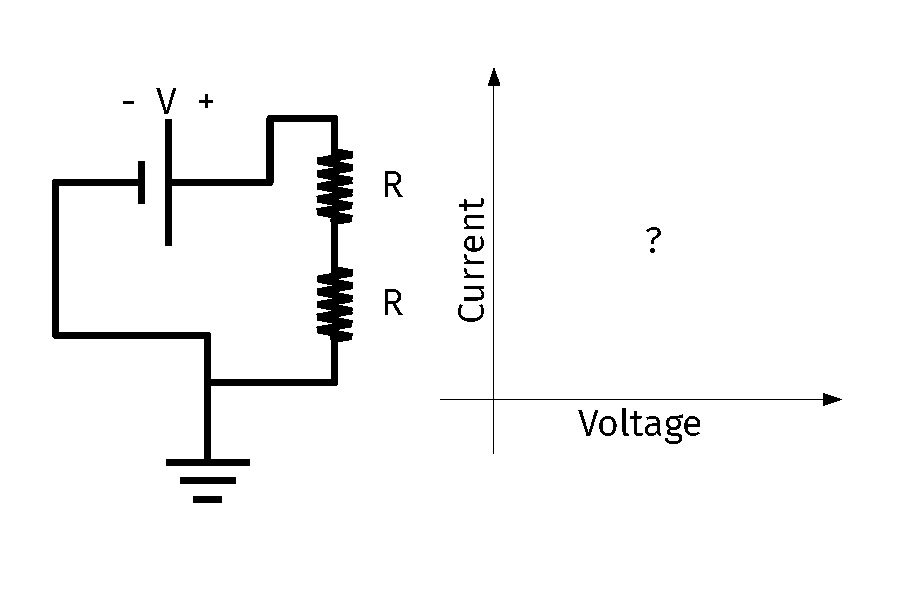
\includegraphics[width=\textwidth,trim=0.5cm 0cm 1cm 0cm,clip=true]{figures/iVCurve2.pdf}
\caption{\label{fig:iVCurve2} Circuits components are represented graphically by iV curves.}
\end{figure}
\end{column}
\begin{column}{0.5\textwidth}
\small
Should the slope now be greater than, less than, or equal to the that of Fig. \ref{fig:iVCurve1}?
\begin{itemize}
\item A: Greater than Fig. \ref{fig:iVCurve1}
\item B: Less than Fig. \ref{fig:iVCurve1}
\item C: Equal to Fig. \ref{fig:iVCurve1}
\item D: Cannot determine.
\end{itemize}
\end{column}
\end{columns}
\end{frame}

\begin{frame}{Graphical Analysis}
\begin{columns}[T]
\begin{column}{0.5\textwidth}
\begin{figure}
\centering
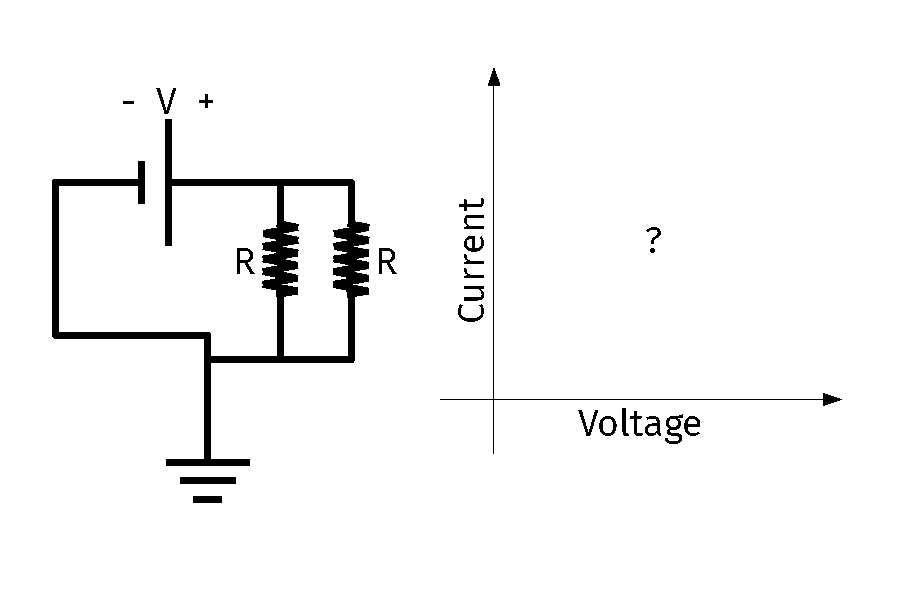
\includegraphics[width=\textwidth,trim=0.5cm 0cm 1cm 0cm,clip=true]{figures/iVCurve3.pdf}
\caption{\label{fig:iVCurve3} Circuits components are represented graphically by iV curves.}
\end{figure}
\end{column}
\begin{column}{0.5\textwidth}
\small
Should the slope now be greater than, less than, or equal to the that of Fig. \ref{fig:iVCurve1}?
\begin{itemize}
\item A: Greater than Fig. \ref{fig:iVCurve1}
\item B: Less than Fig. \ref{fig:iVCurve1}
\item C: Equal to Fig. \ref{fig:iVCurve1}
\item D: Cannot determine.
\end{itemize}
\end{column}
\end{columns}
\end{frame}

\begin{frame}{Graphical Analysis}
\begin{columns}[T]
\begin{column}{0.5\textwidth}
\begin{figure}
\centering
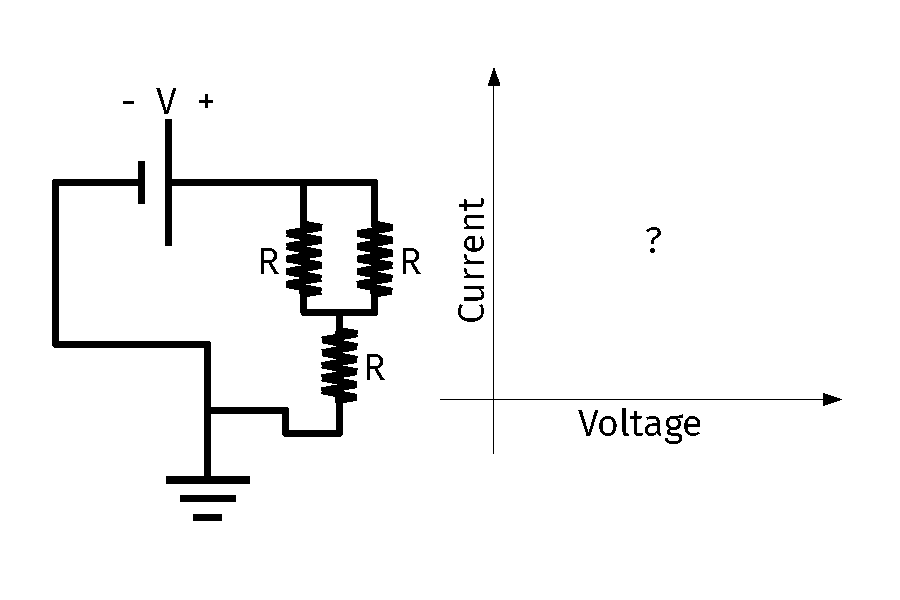
\includegraphics[width=\textwidth,trim=0.5cm 0cm 1cm 0cm,clip=true]{figures/iVCurve4.pdf}
\caption{\label{fig:iVCurve4} Circuits components are represented graphically by iV curves.}
\end{figure}
\end{column}
\begin{column}{0.5\textwidth}
\small
Should the slope now be greater than, less than, or equal to the that of Fig. \ref{fig:iVCurve1}?
\begin{itemize}
\item A: Greater than Fig. \ref{fig:iVCurve1}
\item B: Less than Fig. \ref{fig:iVCurve1}
\item C: Equal to Fig. \ref{fig:iVCurve1}
\item D: Cannot determine.
\end{itemize}
\end{column}
\end{columns}
\end{frame}

\begin{frame}{DC circuit Analysis}
\textbf{Group board exercise:} Solve for the current.
\begin{figure}
\centering
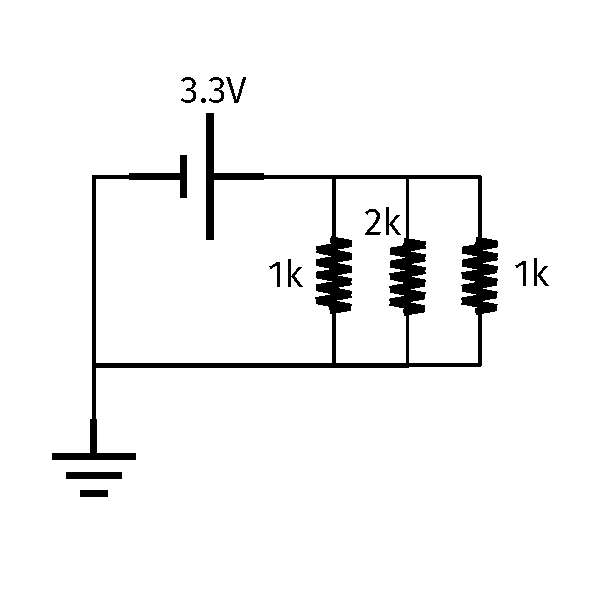
\includegraphics[width=0.5\textwidth]{figures/iVCurve5.pdf}
\caption{\label{fig:iVCurve5} Three resistors in parallel.}
\end{figure}
\end{frame}

\begin{frame}{DC circuit Analysis}
\textbf{Group board exercise:} Solve for the current.
\begin{figure}
\centering
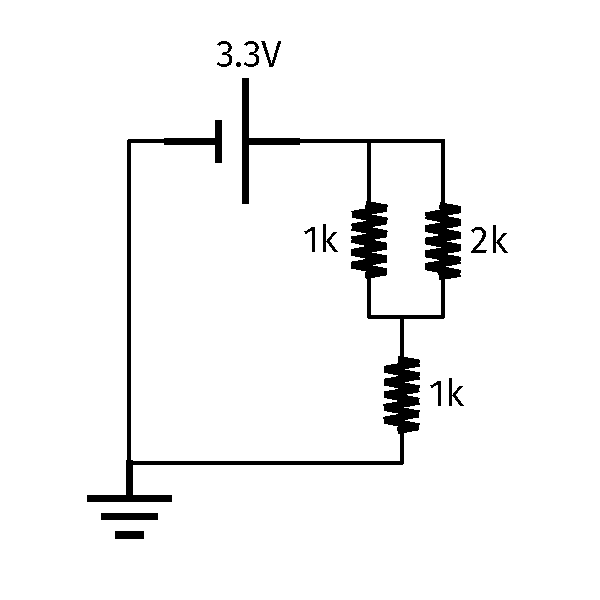
\includegraphics[width=0.5\textwidth]{figures/iVCurve6.pdf}
\caption{\label{fig:iVCurve6} Two resistors in parallel, and in series with a third.}
\end{figure}
\end{frame}

\begin{frame}{DC circuit Analysis}
\textbf{Group board exercise:} Solve for the current.
\begin{figure}
\centering
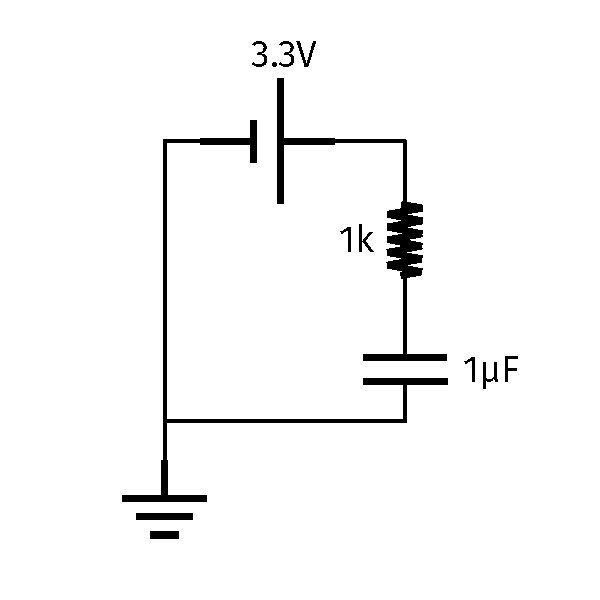
\includegraphics[width=0.5\textwidth]{figures/iVCurve7.pdf}
\caption{\label{fig:iVCurve7} A resistor in series with a capacitor...}
\end{figure}
\end{frame}

\begin{frame}{DC circuit Analysis}
Using Kirchhoff's loop rule:
\begin{align}
V - iR - QC^{-1} &= 0 \\
Q_0 &= CV \\
\tau &= RC \\
\tau \dot{Q} + Q &= Q_0
\end{align}
\textbf{Group board exercise:} Show that the solution for the charge on the capacitor is
\begin{equation}
Q(t) = Q_0 \left(1 - \exp(-t/\tau)\right)
\end{equation}
Take the derivative of both sides to find the current versus time.  Graph the current.
\end{frame}

\begin{frame}{DC circuit Analysis}
So we see that the current is an exponential function:
\begin{equation}
i(t) = i_0 e^{-t/\tau}
\end{equation}
($i_0 = V/R$, the initial current).  What is the current in a circuit with a 1k resistor and a 1 nF capacitor after 3 $\mu$s, if the voltage is 5 V?
\begin{itemize}
\item A: 0.25 mA
\item B: 0.5 mA
\item C: 1.0 mA
\item D: 2.0 mA
\end{itemize}
\end{frame}

\begin{frame}{DC circuit Analysis}
So we see that the current is an exponential function:
\begin{equation}
i(t) = i_0 e^{-t/\tau}
\end{equation}
($i_0 = V/R$, the initial current).  Thinking of the same circuit: when is the current 0.0 mA?
\begin{itemize}
\item A: 3 microseconds
\item B: 30 microseconds
\item C: 300 microseconds
\item D: never
\end{itemize}
\end{frame}

\section{Current}

\begin{frame}{JITT 1.8}
\begin{enumerate}
\item Car batteries are rated in ampere-hours (A h). To what physical quantity do ampere-hours correspond (voltage, current, charge, energy, power,...)?
\item When working with high-power electric circuits, it is advised that whenever possible, you work “one-handed” or “keep one hand in your pocket.” Why is this a sensible suggestion?
\item Does the resistance of an object depend on the path current takes through it? Consider, for example, a rectangular bar—is its resistance the same along its length as across its width?
\item How many electrons flow through a point in a wire in 3.00 s if there is a constant current of I = 4.00 A ?
\end{enumerate}
\end{frame}

\begin{frame}{JITT 1.8}
\textbf{Car batteries are rated in ampere-hours (A h). To what physical quantity do ampere-hours correspond (voltage, current, charge, energy, power,...)?} \\
``They are rated to charge.'' \\
``1 ampere an hour is equal to 3600 coulomb.'' \\
``Ampere hours equals voltage.''
\end{frame}

\begin{frame}{JITT 1.8}
\textbf{When working with high-power electric circuits, it is advised that whenever possible, you work “one-handed” or “keep one hand in your pocket.” Why is this a sensible suggestion?} \\
``Keep you grounded.'' \\
``So you never complete the current your working with so you are not electrocuted.'' \\
``to keep you grounded, your body has a lot more resistance, and you can't complete the circuit when you only work with one hand.''
\end{frame}

\begin{frame}{JITT 1.8}
\textbf{Does the resistance of an object depend on the path current takes through it? Consider, for example, a rectangular bar—is its resistance the same along its length as across its width?} \\
``yes, the resistance along the length would be greater than that along the width.'' \\
``resistance depends on the path you take through and object since the equation R=p(L/A) depends on a length L to find Resistance.  The resistance is not the same when you go through the length and width. The length would produce a higher resistance.''
``Yes it still has the same resistance.''
\end{frame}

\begin{frame}{JITT 1.8}
\textbf{How many electrons flow through a point in a wire in 3.00 s if there is a constant current of I = 4.00 A ?} \\
\begin{itemize}
\item A: $6 \times 10^{18}$
\item B: $6 \times 10^{19}$
\item C: $6 \times 10^{20}$
\item D: $6 \times 10^{21}$
\end{itemize}
\end{frame}

\begin{frame}{Current}
\underline{Notions of current:}
\begin{itemize}
	\item $I = \frac{\Delta Q}{\Delta t}$ - The derivative of charge
	\item The \textit{movement} of electrons
	\item The \textit{flow} of charge
	\item Number of Coulombs per second (1 Amp = C/s)
\end{itemize}
\underline{There is an interesting problem with the notion of current} \underline{as movement of charges.} \\ \vspace{0.5cm}
\begin{columns}[T]
\begin{column}{0.5\textwidth}
Speed of typical electronic signals: $\approx 10^{8}$ m/s
\end{column}
\begin{column}{0.5\textwidth}
Typical speed of actual charges passing through a conductor under voltage: $\approx 10^{-4}$ m/s
\end{column}
\end{columns} \vspace{0.25cm}
\textbf{Since there is a 12 order of magnitude range, it's probably a good idea to ponder...}
\end{frame}

\begin{frame}{Current}
\small
Are the electrons colliding/interacting to form electrical signals?  Or just moving all together?
\begin{figure}
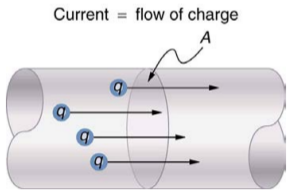
\includegraphics[width=0.5\textwidth]{figures/current1.png}
\caption{\label{fig:current1} The \textit{drift velocity} is the average velocity of an electron, and current is derived from this average velocity.}
\end{figure}
\url{https://youtu.be/8dgyPRA86K0}
\end{frame}

\begin{frame}{Current}
So we see how electrical signals can move near the speed of light, but we measure the movements of electrons in circuits to be slow.  Can we make a calculation to understand the speed of the electrons? \\ \vspace{0.5cm}
\begin{figure}
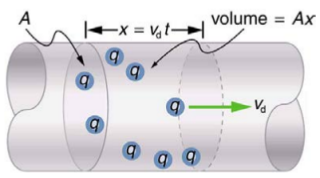
\includegraphics[width=0.5\textwidth]{figures/current3.png}
\caption{\label{fig:current3} Consider the volume $V$ of conductor with cross-sectional area $A$ and length $\Delta x$, having $n$ free electrons per unit volume.}
\end{figure}
\end{frame}

\begin{frame}{Current}
An \textbf{amp} is one \textit{Coulomb} per \textit{second}.  The definition of current is
\begin{equation}
I = \frac{\Delta Q}{\Delta t} = \frac{qnA\Delta x}{\Delta t} = q n A v_{\rm d}
\end{equation}
Solving for drift velocity:
\begin{equation}
v_{\rm d} = \frac{I}{q n A}
\end{equation}
Suppose our conductor is a wire with radius $r$ and $A = \pi r^2$.  Substituting,
\begin{equation}
v_{\rm d} = \frac{I}{\pi q n r^2}
\end{equation}
Remember that $q = 1.6 \times 10^{-19}$ C, and $n$ is the number of free electrons \textit{per atom per unit volume}.  How do we get this number?
\end{frame}

\begin{frame}{Current}
\textbf{Number density}: The total number of objects in a system is equal to the \textit{number density} times the volume of the system.
\begin{equation}
N = nV
\end{equation}
\begin{itemize}
\item N: Total number
\item n: \textit{number density}
\item V: Volume
\end{itemize}
\end{frame}

\begin{frame}{Current}
\textbf{Example:} \alert{Number of Stars in the Milky Way}.  How many stars are in our galaxy?  Assume the galaxy is a disk of height $h$ and radius $r$.  We observe $n$ stars per unit volume.
\begin{itemize}
\item $r$ = $50 \times 10^3$ \textit{light-years}
\item $h = 2 \times 10^3$ \textit{light-years}
\item $n = 10^{-2}$ \textit{light-year} $^{-3}$
\end{itemize}
\begin{enumerate}
\item Compute the volume in \textit{light-years}$^3$
\item Multiply the volume by the number density to obtain the total number.
\item Compare the result with others' results.
\end{enumerate}
\end{frame}

\begin{frame}{Current}
\small
How many \textbf{conduction} electrons are there in a cube of copper that is 1 micron (1 $\mu$m = $10^{-6}$ m) on a side?
\begin{itemize}
\item Copper has a density of 8.8 grams per cubic centimeter.
\item Copper has an atomic weight of 63.54 grams per mole.  (\textit{Do you remember what a mole is?}).
\item There are $N_A = 6.02 \times 10^{23}$ atoms per mole.
\item Only one electron per atom of copper is a conduction electron.
\end{itemize} \hrulefill
\begin{enumerate}
\item Divide the density by the atomic weight.  What are the units?
\item Multiply by $N_A$ (Avogadro's number).  What are the units?
\item Convert the units from $cm^{-3}$ to $\mu m^{-3}$.
\end{enumerate}
\end{frame}

\begin{frame}{Current}
\textbf{Number density}: Let's examine copper, a common wire material with one free electron per atom.  Copper has a density of 8800 kg/m$^3$, and $0.06354$ kg/mol.  There are $6.02 \times 10^{23}$ atoms/mol.  How many free electrons per m$^3$ of copper? (Remember that there is only one conduction electron per copper atom).
\begin{itemize}
\item A: $10^{26}$ free electrons per m$^3$
\item B: $10^{27}$ free electrons per m$^3$
\item C: $10^{28}$ free electrons per m$^3$
\item D: $10^{29}$ free electrons per m$^3$
\end{itemize}
\end{frame}

\begin{frame}{Current}
Consider a copper wire with radius $r = 2.053$ mm that is carrying 20.0 A of current.  Using $q = 1.6\times 10^{19}$, and $n = 8.34 \times 10^{28}$ electrons/m$^3$, and $v_{\rm d} = I/(\pi q n r^2)$, compute the drift velocity of charge in the wire.  \textit{This is a common situation in household wiring.}
\begin{itemize}
\item A: $10^{-1}$ m/s
\item B: $10^{-2}$ m/s
\item C: $10^{-3}$ m/s
\item D: $10^{-4}$ m/s
\end{itemize}
\end{frame}

\begin{frame}{Current}
\textbf{Drift speed vs. signal speed}.  Given that the electrons move at 1 mm/s, how is it that electric signals move at $10^8$ m/s? \\ \vspace{1cm}
\textbf{Electrical signals are \alert{waves} of charge}: \\ \url{https://phet.colorado.edu/en/simulation/legacy/wave-on-a-string}
\end{frame}

\begin{frame}{Current}
\textbf{Resistivity} $\rho$ and \textbf{conductivity} $\sigma$ are intrinsic properties of materials, and they are reciprocals of each other:
\begin{equation}
\rho = 1/\sigma
\end{equation}
Let $\vec{J}$ be the \textit{current density}.  The most general form of Ohm's law is
\begin{equation}
\boxed{
\vec{J} = \sigma \vec{E}}
\end{equation}
Let's assume that current is flowing down a conductor of length $L$ and cross-sectional area $\vec{A}$, parallel to $\vec{E}$.  Integrate both sides:
\begin{align}
I &= \sigma \int \vec{E} \cdot \vec{dA} = E A = \frac{V}{L} A \\
V &= \frac{L \rho}{A} I = I R
\end{align} 
\end{frame}

\begin{frame}{Current}
Thus, the \textit{resistance} of an object is 
\begin{equation}
R = \frac{L \rho}{A}
\end{equation}
The resistivity has units of Ohm meters.  Which of the following is true of a conductor?
\begin{itemize}
\item A: Lengthening it increases the resistance, and widening it increases the resistance.
\item B: Lengthening it decreases the resistance, and widening it increases the resistance.
\item C: Lengthening it increases the resistance, and widening it decreases the resistance.
\item D: Lengthening it decreases the resistance, and widening it decreases the resistance.
\end{itemize}
\end{frame}

\begin{frame}{Current}
Thus, the \textit{resistance} of an object is 
\begin{equation}
R = \frac{L \rho}{A}
\end{equation}
Suppose the length of a conductor is doubled, and the area is quadrupled.  By how much does the resistance change?
\begin{itemize}
\item A: It decreases by a factor of two.
\item B: It decreases by a factor of four.
\item C: It increases by a factor of two.
\item D: It increases by a factor of four.
\end{itemize}
\end{frame}

\begin{frame}{Current}
What is the resistance of a 1 meter-long wire with area 3 mm$^2$ that made from a metal that has $\rho = 10^{-7}$ $\Omega$ m?
\begin{itemize}
\item A: 0.01 Ohms
\item B: 0.1 Ohms
\item C: 1.0 Ohms
\item D: 10.0 Ohms
\end{itemize}
\end{frame}

\begin{frame}{Current}
\begin{figure}
\centering
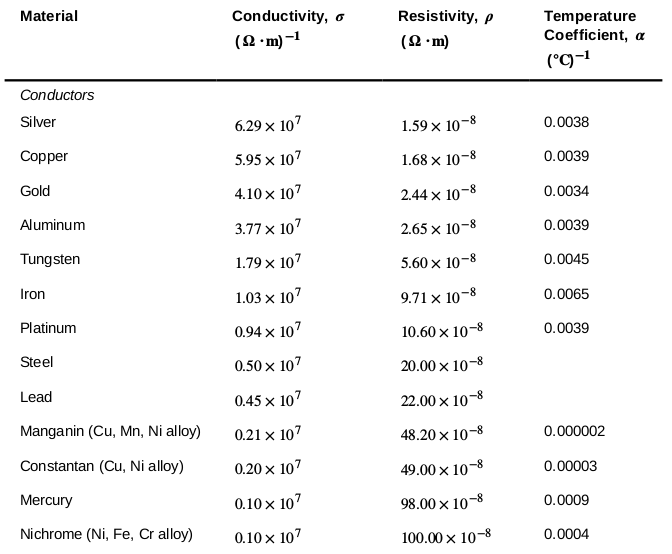
\includegraphics[width=0.8\textwidth]{figures/resist.png}
\caption{\label{fig:resist} Resistivities of various metals.}
\end{figure}
\end{frame}

\begin{frame}{Current}
Like the expansion of metals with increasing temperature, \textit{resistivity has a temperature dependence.}  Let $\Delta T = T - T_0$, with $T_0 = 20.0$ C.
\begin{equation}
\rho = \rho_0 \exp \left( \alpha \Delta T \right)
\end{equation}
Using a Taylor series around $\Delta T = 0$, we find
\begin{equation}
\rho(T) \approx \rho_0 \left(1 + \alpha \Delta T \right)
\end{equation}
\end{frame}

\begin{frame}{Current}
\begin{figure}
\centering
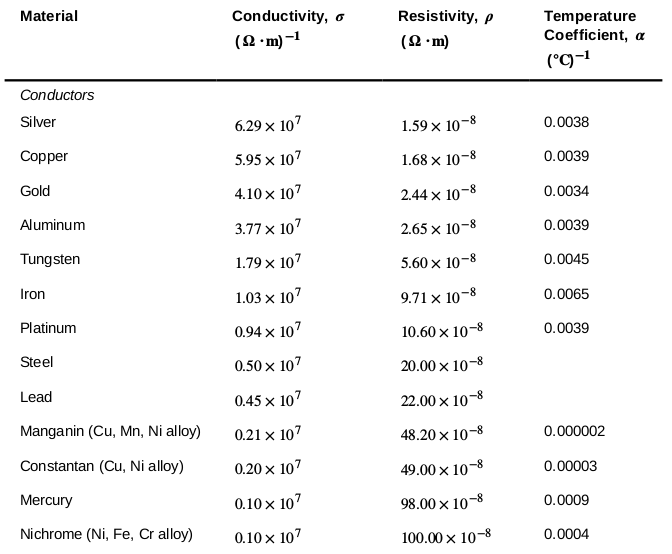
\includegraphics[width=0.7\textwidth]{figures/resist.png}
\caption{\label{fig:resist2} Resistivities of various metals.  Notice the temperature coefficients are small, so the Taylor series is justified.}
\end{figure}
\end{frame}

\begin{frame}{Current}
Consider a copper wire that has a resistance of 0.1 Ohms at 20 degrees C.  What will be the resistance of the wire at 40 degrees C, if the temperature coefficient of copper resistivity is 0.004?
\begin{itemize}
\item A: 0.104 Ohms
\item B: 0.108 Ohms
\item C: 0.112 Ohms
\item D: 0.116 Ohms
\end{itemize}
\end{frame}

\begin{frame}{Current}
Consider a copper wire that has a resistance of 5 Ohms at 20 degrees C.  What will be the resistance of the wire at 50 degrees C, if the temperature coefficient of copper resistivity is 0.004?
\begin{itemize}
\item A: 4.8 Ohms
\item B: 5.0 Ohms
\item C: 5.6 Ohms
\item D: 6.0 Ohms
\end{itemize}
\end{frame}

\begin{frame}{Current}
Given that we found a 12\% increase in the resistance of the wire in the prior example, what would happen to the voltage delivered to a device at the other end of that wire?
\begin{itemize}
\item A: It would be unaffected.
\item B: It would decrease by 12 percent.
\item C: It would increase by 12 percent.
\item D: It would decrease by 6 percent.
\end{itemize}
\textit{So you can see why we don't do DC power transmission over long distances.}
\end{frame}

\section{Conclusion}

\begin{frame}{Unit 4 Summary}
\textbf{Reading: Chapters 7, 9, and 10}
\begin{enumerate}
\item \alert{Voltage and Capacitance}
\item Ohm's Law
\item DC circuits
\end{enumerate}
\end{frame}

\section{Answers}

\begin{frame}{Answers}
\small
\begin{columns}[T]
\begin{column}{0.5\textwidth}
\begin{itemize}
\item $\vec{E} = \frac{kq}{r^2}\hat{r}$
\item $\vec{E} = \frac{2k\lambda}{r}$
\item $\vec{E} = -a\hat{i}$
\item $\vec{E} = -a\hat{i}-b\hat{j}$
\item 40 keV
\item 1 MV
\item about 1 nm
\item $1.2 \times 10^{-13}$ J
\item 0.75 MeV
\item 0.375 MV
\end{itemize}
\end{column}
\begin{column}{0.5\textwidth}
\begin{itemize}
\item ...
\end{itemize}
\end{column}
\end{columns}
\end{frame}

\end{document}
